\section{Muon Decay at \mueee}
\mueee \cite{Blondel:2013ia} is a proposed experiment, currently under construction, that will look for the decay of $\mu^+ \rightarrow e^+ e^+ e^-$, which violates lepton flavour.
This experiment will operate at the Paul Scherrer Institute (PSI) in Switzerland, and is currently taking data in its first phase for 2015-2016.
A second phase for 2017 and beyond is planned, and the details of the phases are covered in this section. 
Lepton flavour violating (LFV) decays are allowed within the SM once one includes the neutrino masses.
Since we see LFV processes in the nuetrino sector, due to nuetrino mixing, it is not unreasonable to expect that there may also be new physics that violates lepton number in the charged lepton sector.
\mueee is aiming to find BSM LFV by investigating such $\mu^+$ decays.
The SM process for $\mu^+ \rightarrow e^+ e^+ e^-$ is show in Fig. \ref{fig:mu_eee_SM}.
\begin{figure}[h]
    \centering
    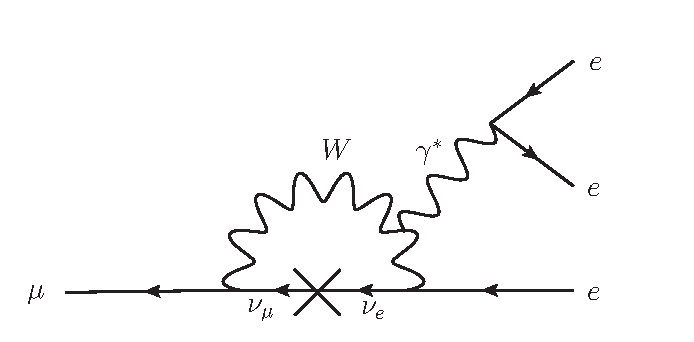
\includegraphics[height = 1.5in]{Figures/feynman_diagrams/mu_eee_SM.eps}
    \caption[$\mu^+ \rightarrow e^+ e^+ e^-$ lepton flavour violating decay through neutrino oscillation.]{$\mu^+ \rightarrow e^+ e^+ e^-$ LFV decay with a muon neutrino oscillating to an electron neutrino. This process is heavily suppressed due to the neutrino oscillation required.}
    \label{fig:mu_eee_SM}
\end{figure}
For this process, the required neutrino oscillation which mediates the lepton flavour violating component suppresses the branching ratio of this process, so much so that $\textrm{BR}(\mu^+ \rightarrow e^+ e^+ e^-) \ll 10^{-50}$.
This is an unobservably low decay rate, and so any decays of this form will almost certainly be a sign for new physics.

New physics may come in the form of new particles that can mediate these loops without a penalty like the neutrino mixing, if it is to be observed.
This could be in the form of supersymmetric particles in a loop, or other particles which add couplings to muons and electrons.
It is also possible that a new mediator adds observable contributions at tree level.

The current experimental limits on the branching ratio of various muon decay processes is shown in Table \ref{table:mu_br_limits}.

\begin{table}[h]
\label{table:mu_br_limits}
\begin{center}
\begin{tabular}{|l|l|l|} \hline
Decay Channel & Experiment & Branching Ratio \\ \hline
$\mu \rightarrow e \gamma$ & \mega & $< 1.2\times 10^{-11}$ \\
& \meg & $< 2.4\cdot 10^{-12}$ \\ \hline
$\mu \rightarrow eee$ & \sindrum & $< 1.0\times 10^{-12}$ \\ \hline
$\mu~Au\rightarrow e~Au$ & \sindrumii & $< 7\times 10^{-13}$ \\ \hline
\end{tabular}
\end{center}
\caption{Branching ratio limits on muon decay from various experiments as given in \cite{Blondel:2013ia}.}
\end{table}

Note that all of these upper limits are on the order of $10^{-10} - 10^{-13}$.
Any future experiments must examining these decay modes must be sensitive to branching ratios at least as small as the upper limits here.
For this reason, \mueee is attempting to reach branching ratios down to $10^{-16}$ for the $\mu \rightarrow eee$ process.
